\documentclass[uplatex, dvipdfmx, unicode]{beamer}
\usetheme{CambridgeUS}
\usepackage{amsmath, amssymb}

\title{入出力の話}
\author{@leno3s}
\date{\today}
\institute{leno3s.net}

\begin{document}
\maketitle

\begin{frame}{もくじ}
  \tableofcontents
\end{frame}

\begin{frame}{今日の目標}
  \begin{itemize}
    \item{標準入出力を理解する.}
    \item{リダイレクトを用いたファイルの入出力ができる.(重要)}
    \item{シェル芸への思想を理解する.(発展)}
  \end{itemize}
  

\end{frame}

\begin{frame}{対象}
  \begin{itemize}
    \item{簡単なCLIでの操作(ls, cd, cat, echo, ...)はわかる}
    \item{競技プログラミングの簡単な問題が解ける}
  \end{itemize}

\end{frame}

\section{CUI使ってますか?}
\begin{frame}
  \centering
  \Huge{CUI使ってますか?}
\end{frame}

\begin{frame}
  \centering
  \Huge{使ってる人✋}
\end{frame}

\begin{frame}
  \centering
  \Huge{使ってない人✋}
\end{frame}

\begin{frame}
  \centering
  \Huge{わからない人✋}
\end{frame}

\begin{frame}
  \centering
  \Huge{はい}
\end{frame}

\begin{frame}
  というわけでCUIの話をします.
\end{frame}

\begin{frame}
  そもそもCUIとは?
  \begin{itemize}
    \item{Charcter User Interface}
    \item{グラフィカルでない, 文字を基本としたインターフェース}
  \end{itemize}
\end{frame}

\begin{frame}
  \centering
  \Huge{↓これとか,} \\

  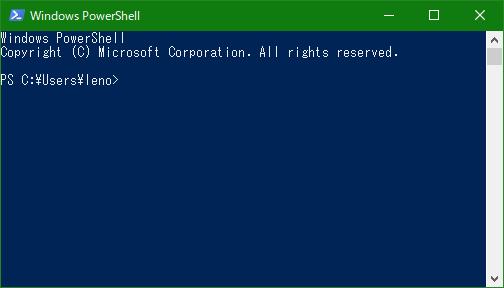
\includegraphics[keepaspectratio, scale=.5]{./img/ps.png}
\end{frame}

\begin{frame}
  \centering
  \Huge{↓これとか.} \\

  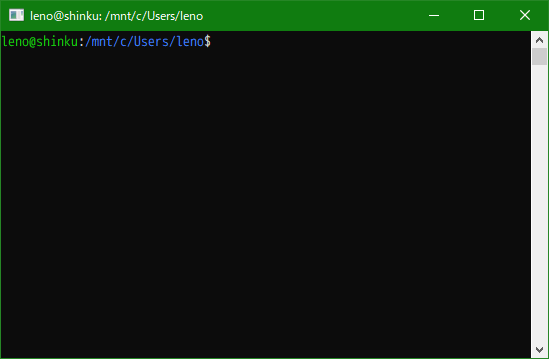
\includegraphics[keepaspectratio, scale=.5]{./img/bash.png}
\end{frame}

\begin{frame}
  普段からこんな感じで使っていると思います.
  
  \centering
  ここに画像
\end{frame}

\begin{frame}
  競プロではあるある風景ですね. (ほんまか?)
\end{frame}

\begin{frame}
  ---ところでそろそろICPC予選ですね.
\end{frame}

\begin{frame}
  ICPCでは, テストケースがテキストファイルで与えられます.\\
  (提出も, 出力結果のテキストファイルです.)
\end{frame}

\begin{frame}{}
  \centering
  \Huge{この形式のコンテストに参加した事がある人✋}
\end{frame}

\begin{frame}{}
  fopen()とか使うのめんどくさいよね... \\
  (普段みたいにcin/cout, scanf/printfでやりたいよね)
\end{frame}

\begin{frame}{というわけで}
  標準入出力について, お話します.
\end{frame}

\section{標準入出力って?}
\begin{frame}
  \centering
  \Huge{標準入出力についてご存知の人✋}
\end{frame}

\begin{frame}
  \begin{quote}
    標準ストリーム(英: standard streams)とは、UNIXやUnix系オペレーティングシステム (OS) において、プログラムの活動実体であるプロセスとその実行環境(通常は端末)の間の接続として、(プロセスから見ると)あらかじめ確立されている入出力チャネル(パイプ (コンピュータ))である。OSのカーネルではなくシェルで実装されている機能だが、広く使われているため標準化されている。UNIXやUnix系OSでは3つの入出力があり、標準入力(英: standard input)、標準出力(英: standard output)、標準エラー出力(英: standard error)である。
  \end{quote}
  \small{標準ストリーム - Wikipedia\footnote{https://ja.wikipedia.org/wiki/標準ストリーム}より.}
\end{frame}

\begin{frame}
  \centering
  \Huge{('$\mathrm{\omega}$')????????}
\end{frame}

\begin{frame}
  \begin{quote}
    標準ストリームとは、UNIXやUnix系オペレーティングシステム (OS) において、
    \alert{プログラムの活動実体であるプロセスとその実行環境(通常は端末)の間の接続}として、
    (プロセスから見ると)あらかじめ確立されている\alert{入出力チャネル}(パイプ (コンピュータ))である。 \\
    OSのカーネルではなくシェルで実装されている機能だが、広く使われているため標準化されている。
    UNIXやUnix系OSでは3つの入出力があり、\alert{標準入力、標準出力、
    標準エラー出力}である。
  \end{quote}
\end{frame}

\begin{frame}{重要ポイント}
  \begin{itemize}
    \item{なんかプロセス間の通信に使ってるらしい}
    \item{標準入力, 出力, エラー出力がある}
  \end{itemize}
\end{frame}

\section{/dev/ptsの話}

\begin{frame}
  \Huge{\alert{/dev/pts/の話}}
\end{frame}

\begin{frame}
  \Large{\alert{ここからLinux/Unix基準の話をします}} \\
  \vspace{0.2in}

  \normalsize
  環境の無い人は WSL や MSYS2 でも大丈夫, Cygwinは確認してない \\
  コマンド交えつつ話すので, 手元で実行してね
\end{frame}

\begin{frame}{/dev/って?}
  /以下のディレクトリの1つ \\
  \vspace{0.2in}
  ここにls /devの画像
\end{frame}

\begin{frame}{/dev/って?}
  \begin{itemize}
    \item{\alert{dev}iceのdev}
    \item{装置の意味}
    \item{Linux/Unixで, デバイスのための疑似ファイルが置かれる}
  \end{itemize}
\end{frame}

\begin{frame}{疑似ファイルの例}
  \begin{itemize}
    \item{/dev/stdin}
    \item{/dev/stdout}
    \item{/dev/stderr}
    \item{/dev/null}
    \item{/dev/zero}
    \item{/dev/(u)random}
  \end{itemize}
  \vspace{0.2in}
  など\ 実際はもっといっぱいある\footnote{\$ ls /dev/ して見れる 見てね}
\end{frame}

\begin{frame}{/dev/stdinを追ってみる}
  \$ ls -al /dev/stdin でstdinの情報が見れる \\
  \vspace{0.2in}
  ここに画像 \\
  どうやら/proc/self/fd/0へのリンクらしい \\
\end{frame}

\begin{frame}{/dev/stdinを追ってみる}
  同様に\$ ls -al /proc/self/fd/0 する \\
  \vspace{0.2in}
  ここに画像 \\
  /dev/pts/1 へのリンクらしい(数字部は人によって違います)
\end{frame}

\begin{frame}
  同様に\$ ls -l /dev/pts/1 する \\
  ここに画像 \\
  これが本体, 数字部は...後で説明します.
\end{frame}

\begin{frame}{ttyコマンド}
  実はこの番号を調べるコマンドがある \\
  \vspace{0.2in}
  \$ tty \\
  /dev/pts/1
\end{frame}

\begin{frame}{ttyコマンド}
  もう一つウィンドウを開いて\$ ttyしてみる\\
  \vspace{0.2in}
  \$ tty \\
  /dev/pts/2
\end{frame}

\begin{frame}{ttyコマンド}
  \centering
  \alert{\Huge{!!!違う番号になった!!!}}
\end{frame}

\begin{frame}{ttyコマンド}
  ポイント
  \begin{itemize}
    \item{この番号によってウィンドウを識別している}
    \item{なんかすごいぎじゅつでウィンドウごとにstdin/out/errの番号が変わる}
  \end{itemize}
\end{frame}

\subsection{補足}
\begin{frame}{補足}
  Q. ttyって何よ \\
  A. \alert{T}ele \alert{TY}pewriter
\end{frame}

\begin{frame}{補足}
  印刷電信機, 昔はこれで通信をしていた. $\rightarrow$ 通信端末

  \centering
  ここにテレタイプ端末の画像
\end{frame}

\begin{frame}{補足}
  ユーザーがコマンドを打ち込み, 結果を出力する様子がこれと似ている

  \ \ $\rightarrow$ 端末, Terminal
\end{frame}

\begin{frame}{補足}
  しかし, 今あるウィンドウは実際の端末ではない\\
  \ \ $\rightarrow$ Pseudo TTY(仮想端末) \\
  \ \ $\rightarrow$ pts
\end{frame}

\begin{frame}{補足}
  \centering
  \Huge
  $\downarrow$ 端末 $\downarrow$
\end{frame}

\begin{frame}
  \centering
  補足終わり
\end{frame}

\subsection{}
\begin{frame}{ここで疑問}
  違う番号の/dev/pts/[0-9]*に書き込みをしたらどうなるのか?
\end{frame}

\begin{frame}{実際にやってみる}
  \begin{itemize}
    \item{vimやnano等での書き込みはできない}
    \item{\$ echo hogeしてもその端末の標準入力へ流れる}
  \end{itemize}
\end{frame}

\begin{frame}{リダイレクト}
  出力先を変えるコマンド(嘘)\footnote{これはシェルの機能であってコマンドではない}がある \\
  \$ echo hoge \alert{$>$ ./out.txt} \\
  で./out.txtへと出力することができる
\end{frame}

\begin{frame}{やってみよう!}
  \$ echo hoge $>$ /dev/pts/2 \\
  (端末の番号は各自変えてね)
\end{frame}

\begin{frame}{やってみよう!}
  できましたか?どうなりましたか?✋
\end{frame}

\begin{frame}{やってみよう!}
  \$ command \alert{$>$ to/file/path} \\
  が標準出力先をto/file/pathへ向けている \\
  $\rightarrow$ ファイルへの保存ができる!
\end{frame}

\begin{frame}{標準入力}
  ちなみに: 入力のリダイレクトもできる
  \tiny{標準入力から待ち受けるコマンド少なくて例示がしづらい...} \\
  \normalsize
  \$ cat $<$ out.txt \\
  \vspace{.2in}
  普段はキーボードから入力を待つところを, ファイルの内容を入力とすることができる. \\
  \ \ $\rightarrow$ !!! 競プロの標準入力では !!! \\
\end{frame}

\begin{frame}{まとめ}
  \$ command $>$ to/file/path \\
  \ \ $\rightarrow$ 標準出力リダイレクト \\
  \vspace{.2in}
  \$ command $<$ to/file/path \\
  \ \ $\rightarrow$ 標準入力リダイレクト \\
\end{frame}

\begin{frame}{まとめ}
  \$ command $<$ input.txt $>$ output.txt \\
  \ \ $\rightarrow$ 入力をinput.txtとし, 出力をoutput.txtへ保存する. \\
  \ \ $\rightarrow$ fopen/fwrite使わなくていい!cin/cout, scanf/printfでいい!
\end{frame}

\section{競プロへの応用}

\begin{frame}
  \centering
  \Huge{競プロへの応用}
\end{frame}

\begin{frame}
  実際にICPCを想定してリダイレクトの演習をします. \\
  けどテストデータ作るのは面倒くさいので, AtCoderの例題でも解いてもらいます. \\
\end{frame}

\begin{frame}
  ここから@\_\_Bactpus\_\_のターン
\end{frame}

\section{発展 : シェル芸}
\begin{frame}
  \centering
  \Huge{発展: シェル芸}
\end{frame}

\begin{frame}{パイプ}
  あるコマンドの出力を次のコマンドの入力として渡す事ができる \\
  \$ echo foge $|$ sed s/f/h/ \\
  hoge

  \small いわゆるシェル芸で頻出
\end{frame}

\begin{frame}{シェル芸とは?}
  ``シェル芸 とは、主にUNIX系オペレーティングシステムにおいて「マウスも使わず、ソースコードも残さず、
  GUIツールを立ち上げる間もなく、あらゆる調査・計算・テキスト処理を CLI端末へのコマンド入力 一撃で
  終わらせること」である。この技術を持つ人物を シェル芸人 という。''
  \footnote{USP友の会会長・上田隆一による定義}
\end{frame}

\begin{frame}
  \centering
  
\includegraphics[keepaspectratio, scale=.5]{./img/shellgei.png}\\
  \url{https://twitter.com/minyoruminyon}
\end{frame}

\begin{frame}
  興味のある人は過去のシェル芸勉強会の問題集\footnote{\url{https://b.ueda.tech/?page=00684}}を参照するとよい.
\end{frame}

\begin{frame}{簡単な例}
  サイコロ \\
  \$ seq 6 $|$ shuf $|$ head -1 \\
  \vspace{0.2in}

  連番ディレクトリの作成 \\
  \$ mkdir \$(seq -w 14)
  \vspace{0.2in}
  
  FizzBuzz \\
  \$ seq 31 $|$ sed 5$\sim$5cBuzz $|$ sed 3$\sim$3s/[0-9]*/Fizz/
  \vspace{0.2in}

  OSのユーザー数を求める \\
  \$ cat /etc/passwd $|$ awk -F: '$\{\text{print \$1}\}$' $|$ wc -l
\end{frame}

\begin{frame}
  \centering
  \Large
  おわり. \\
  \normalsize
  ご清聴ありがとうございました. \\
  ご意見やマサカリ, 質問は\url{twitter.com/leno3s}へ.
\end{frame}

\end{document}


